%-----------------------------------------------------------------------------------------
\clearpage
\section{Evaluation}
%-----------------------------------------------------------------------------------------
In this section, we provide the description to the performance of the project, along with the illustration of our observation from the outcome of the visualisation. Feedback from a domain expert are also rendered as an evaluation.

\subsection{Results}

\paragraph{Frequency Visualisation}
\paragraph[]{}
The Frequency Visualisation is the basic feature and the primary task in this project. In this visualisation, we aim at providing a parallel view for concordances to display the most frequent words in each version of the translation. As shown in Figure \ref{fig:highlightView}, the colour of blocks differs from each other and the width of blocks represents ranges from the longest to the shortest. And highlight feature allows user to see same terms in each concordance. 

However, from the result in the frequency visualisation, we can tell that the most frequent words in each version are the noise, and stop words such as 'ich' which means 'I' in English, or 'und' which means 'and' in English. These kinds of words are help a little in translation comparison.

\paragraph{Tf-Idf Visualisation}
\paragraph[]{}The Tf-Idf Visualisation is another feature provided in this project. Based on features in Frequency Visualisation, the Tf-Idf Visualisation displays the most important words in the concordance. Therefore, the results of this visualisation is quite different with the Frequency Visualisation. In Figure \ref{fig:tfIdfView}, terms in each concordance changed a lot. As illustrated in Tf-Idf visualisation implementation part, if a word is listed on the top of concordance, it means this word may appear a lot of times in this version of translation, while appearing not many time in other concordance. For example, from Figure \ref{fig:fassung}, the word 'fassung',which means 'composure', in the 1941 version of translation which written by Schwarz, which appears high Tf-Idf value. And from highlight result (by clicking this word), it appears that no other blocks are highlighted, which means the word 'fassung' are not used by other authors. There are several guesses for this result:
\begin{itemize} 	
	\item \textbf{} The word 'fassung' is used more than one times in this translation version. So this is used to translate certain word or express specific meaning. (In this text, it is used to translate 'patience' or express 'the state of being calm and in control of oneself')
	\item \textbf{} This word does not appear in other versions, which can be assumed as special translation techniques are adopted, such as reformulation, adaptation, or compensation. 
	\item \textbf{} This unique outcome is possible aroused by culture influences. Different culture may leads to nuances in linguistic expression. In other words. The author may come from a special region where compared with other places, people used to use different words to express same meaning.
\end{itemize} 

\begin{figure}[H]
	\centering	
	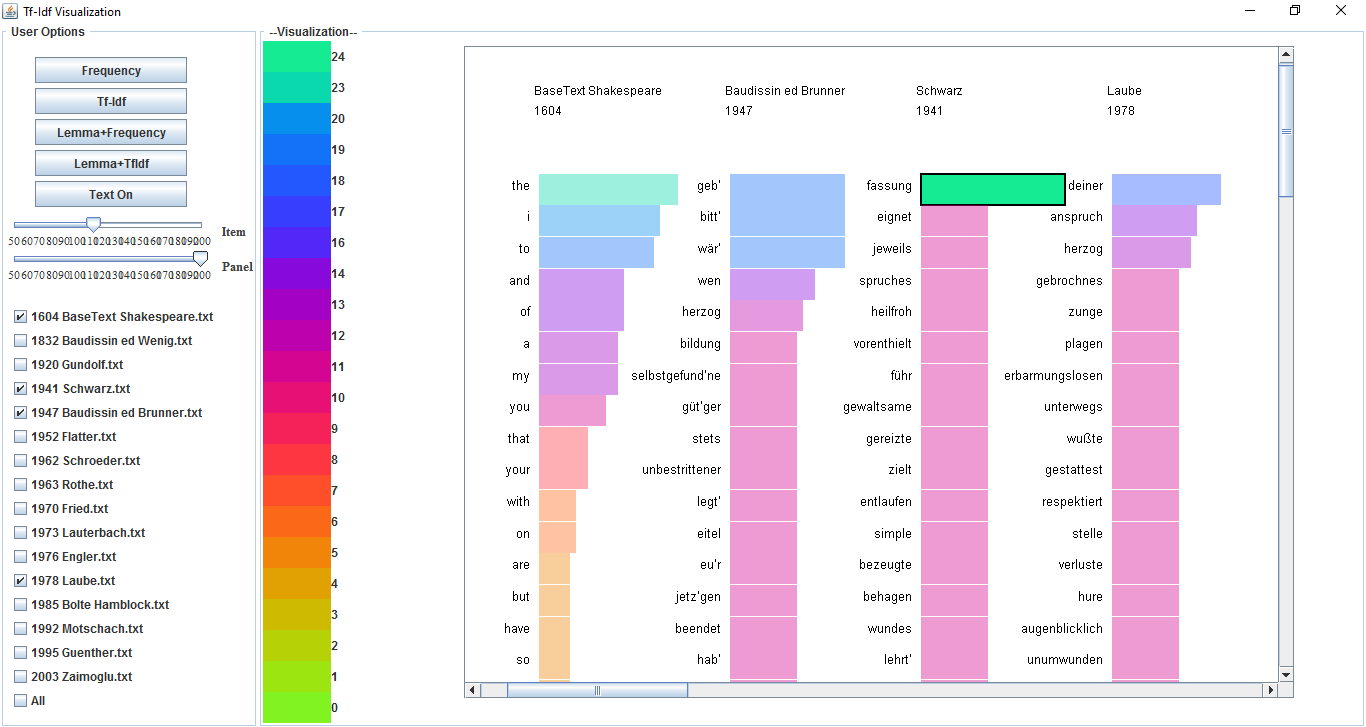
\includegraphics[scale=0.4]{Figs/Fassung}\\[1ex]
	\caption{}
	\label{fig:fassung}
\end{figure} 

\paragraph{Lemma Visualisation}
\paragraph[]{}Lemma Visualisation is generated after applying lemma corpus to process our data. After lemmatisation, words are supposed to change into the original form, namely, the dictionary form (See Implementation chapter to see relevant explanation). This feature is designed to combine same words with different inflected forms.
 For example, the English word 'you' can be translated into 'dir', 'du', 'sie' , 'euch', and 'euch' in German. Figure \ref{fig:youInFreq} is the result after we selecting 'you' in ther base text concordance. However, in Lemma Visualisation, only 'ihr' is highlighted.
 
\begin{figure}[H]
	\centering	
	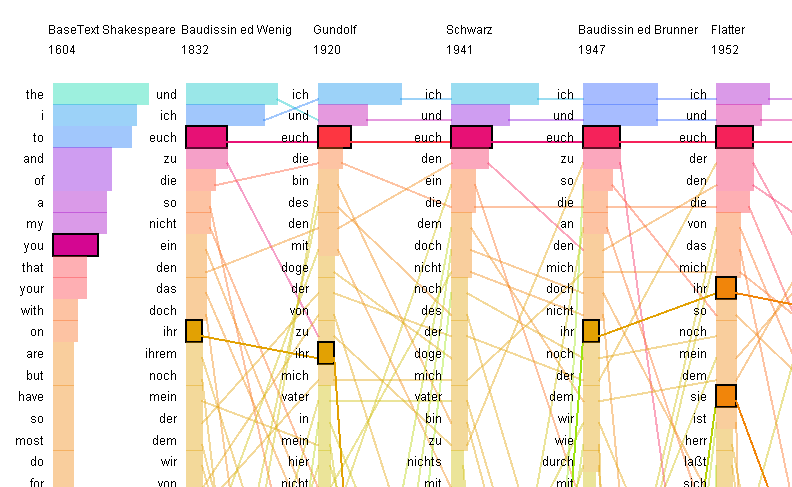
\includegraphics[width=16cm, height=12cm]{Figs/You-In-Frequency}\\[1ex]
	\caption{} After clicking the block of English 'you' in base text, all German translations in other concordances are highlighted, such as  'dir', 'du', 'sie' , 'euch', and 'euch'. Figure \ref{fig:youInLemma} show the example of highlighting 'you' and relevant translation.
	\label{fig:youInFreq}
\end{figure} 
\begin{figure}[H]
	\centering	
	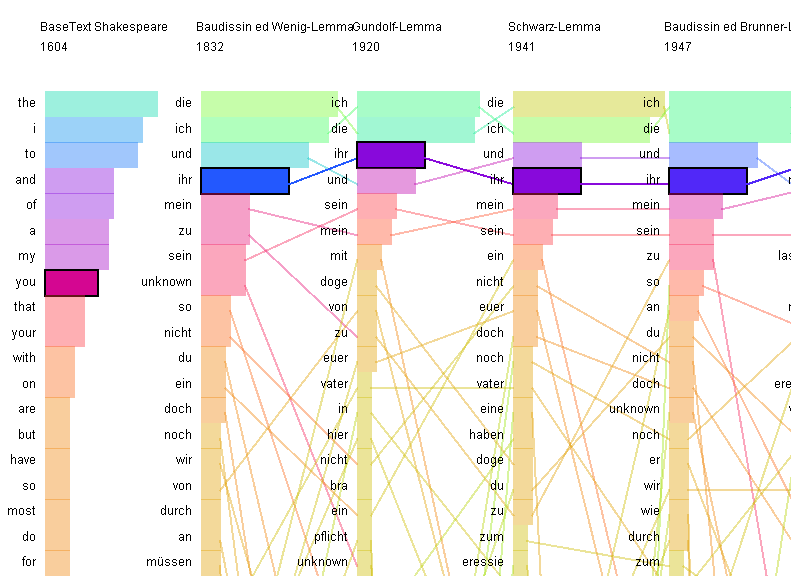
\includegraphics[width=16cm, height=12cm]{Figs/You-In-Lemma}\\[1ex]
	\caption{} After clicking the block of English 'you' in base text, all German translations in other concordances are highlighted, such as  'dir', 'du', 'sie' , 'euch', and 'euch'.
	\label{fig:youInLemma}
\end{figure} 

As a result of lemmatisation, the length of column is shorter in the lemma view than in the frequency view. And the frequency of words are changed. This can be seen from the colour legend in Figure \ref{fig:freqLemmaComp}. Meanwhile, it can be assumed that the variety of words are more obvious. However, more proofs and interpretations need to be probed in the future.

\begin{figure}[H]
	\centering	
	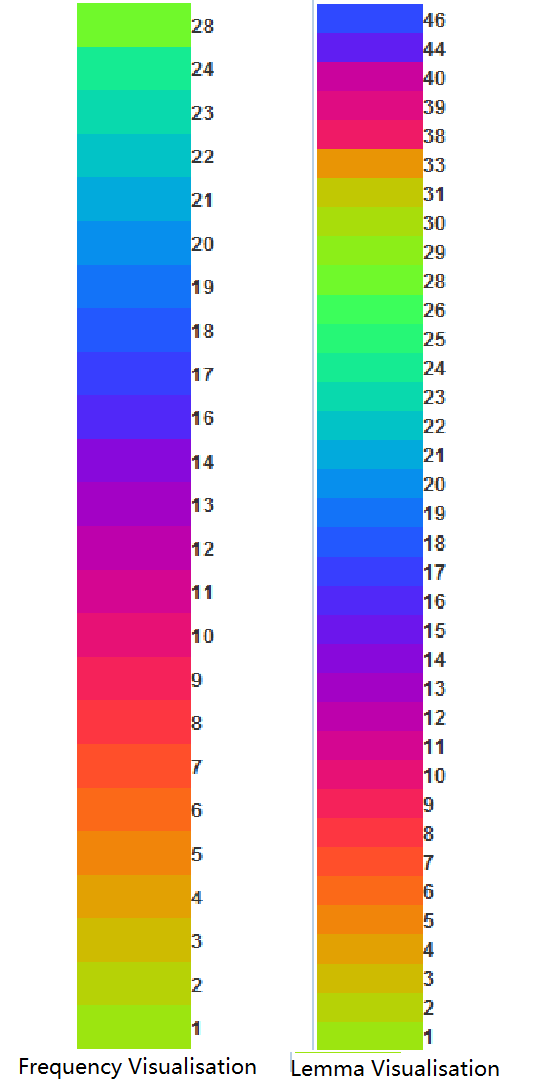
\includegraphics[width=8cm, height=19cm]{Figs/Freq-Lemma-Comparison}\\[1ex]
	\caption{} After combining the inflected form of words, the frequencies are incremented.
	\label{fig:freqLemmaComp}
\end{figure} 

\paragraph{Lemma and Tf-Idf Visualisation}
\paragraph[]{} The last view we rendered is the Lemma and Tf-Idf Visualisation. In this view, both the techniques of lemmatisation and Tf-Idf are utilized to display a parallel translation comparison in the software. From this visualisation, not only can we see the dictionary words, but the stop words are filtered. To prove the advantages of this results, two comparison is necessary:
\begin{itemize} 	
	\item \textbf{Tf-Idf Visualisation vs Lemma and Tf-Idf Visualisation}\\
     The German word 'wen', meaing 'whom' in English, which bears little content information but performs grammar function. In Tf-Idf visualisation of Figure  \ref{fig:tfIdfView}, the word 'wen' ranked on the top of second version from left which is written by Baudissin ed Wenig in 1832\cite{Hotho2005}. However, in Figure \ref{fig:tfIdfLemma}, which applied both lemmatisation techiniques and Tf-Idf algorithm, this word disappear. It can be caused by the reason that the word is combined to the dictionary word of 'wen', which has low Tf-Idf value.
	\item \textbf{Lemma Visualisation vs Lemma and Tf-Idf Visualisation}\\
	If we only apply lemmatisation in the visualisation, stop words are still stay. In Figure \ref{fig:lemmaView}, words such as 'die'('the' in English), 'ich'('I' in English), and 'und'('and' in English) are all considered as stop words \cite{Hotho2005}, which contributes a little in translation studying. In the Lemma and Tf-Idf view, these words are disappeared which is because they are ranked to the bottom. 
\end{itemize}

\subsection{Domain Expert Feedback}

A domain expert, Dr. Tom Cheesman from the College of Art and Humanities at Swansea University, was invited as the user to give feedback for this project. During the meetings, we demonstrated the visualisations and features to him and he gave feedback to the project. The first one was organised on 13th November, 2017. According to the feedback, some features were overwritten and several new features were developed. The second meeting was on 4th December, 2017, in which he gave for new features. 

\subsubsection{Session 1}

At this stage, Frequency Visualisation was finished, along with features such as turn the visualisation on and off, scaling the frame, versions selection, and colour legend are implemented. Dr. Tom Cheesman expressed his interesting by leaning his body to watch closer the laptop. He asked some questions such as 'What the numbers beside colour legend represent?', 'What are the connections?'. He also required to show only base text and three other German translations so that he could understand the alignments. In the feed back, words like 'interesting', 'useful' and 'good' were used a lot. Meanwhile, there are other suggestions were mentioned and discussed, such as filtering stop words and see the most important words, together with show the lemma of the words to decrease inflected words.

\subsubsection{Session 2}

In this stage, according to the feedback Dr. Cheesman gave at the first meeting, we did some changes for the project: utilizing Tf-Idf algorithm in data processing, and using the German lemma corpus to lemmatize the terms. 

In the meeting, Dr. Cheesman express more interests and excitements by saying 'This is good, this is pulling up some interacting stuff', 'This is great...I can play with this'. He showed great interests in the Lemma and Tf-Idf view, and pointed out some remarkable translations such as abbreviation words in the version written by Baudissin ed Brunner in 1947, (See Figure \ref{fig:feedback}). From the view, we can tell that more abbreviation words are used in this version which implies this is a unique translation strategy the author uses. At last, Dr. Cheesman asked for a copy of the tools for assisting his translation studies.

\begin{figure}[H]
	\centering	
	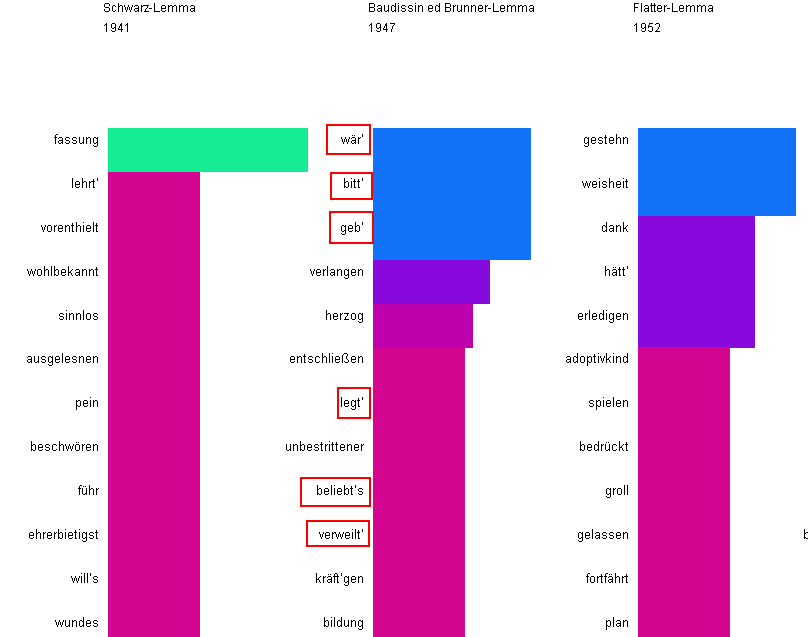
\includegraphics[width=16cm, height=12cm]{Figs/Marking-Feedback}\\[1ex]
	\caption{} After combining the inflected form of words, the frequencies are incremented.
	\label{fig:feedback}
\end{figure} 




